\documentclass[../../../main]{subfiles}
\begin{document}

\section{考察}

\subsection{TMR曲線とMTJ素子の状態}
図\ref{fig:result}に示したTMR曲線をみると、$H>0$のとき抵抗は大きくなり、$H<0$のときは実験1と比較すると小さくなっている。
また、$H>0$の範囲で、抵抗の値は$H$が\SI{15}{mT}前後で最大となりそのごは減少している。
したがって、このMTJ素子は$H>0$の領域では、$H$が\SI{15}{mT}前後で2つの強磁性体の磁化が最も反平行で差が最大となり、その後は磁化が平行になると考えられる。
つまり、ある程度$H$が小さい範囲では一方のみが顕著に磁場の影響を受け磁化が変化し反平行になっているが、
大きくなると両方の磁化が磁場の向きに揃い、平行になっっていくため最終的には磁場が0の状態に比べて小さくなったと考えられる。
一方で$H<0$の領域ではともに磁化が平行で差が小さくなり、抵抗が小さくなったと考えられる。

また、スピン分極率は\SI{65.90}{\%}であり、MTJ素子はアップスピンとダウンスピンがほぼ同程度ずつ含まれていると考えられる。

\subsection{結晶中のDOS}
図\ref{fig:tmr-dos}ではDOSは楕円弧を描くように閉じている。
量子力学的考察では、3次元の井戸型ポテンシャルの自由粒子の波動関数を考えると、
シュレディンガー方程式
\begin{equation}
	-\dfrac{\hbar^2}{2m}\Delta \psi(\bm{r}) = \epsilon_n \psi(\bm{r})
\end{equation}
を解くことになる。
これを解くと、
\begin{align}
	\psi_{n_1,n_2,n_3} (\bm{r}) & = \left(\dfrac{2}{L}\right)^{3/2} \sin\left(\dfrac{n_1\pi x}{L}\right)   \sin\left(\dfrac{n_2\pi y}{L}\right) \sin\left(\dfrac{n_3\pi z}{L}\right) \\
	\epsilon_{n_1,n_2,n_3}      & = \dfrac{\pi^2 \hbar^2}{2mL^2}\left(n_1^2 + n_2^2 + n_3^2\right)                                                                                   \\
	\bm{k}                      & = \dfrac{\pi}{L} \bm{n} \label{eq:3d-free-particle}
\end{align}
となり、このときの状態密度$D(\epsilon)$ ($\epsilon \geq 0$)は
\begin{equation}
	D(\epsilon) = L^3 \left(\dfrac{2m}{\hbar^2}\right)^{3/2} \dfrac{\sqrt{\epsilon}}{4\pi^2}
\end{equation}
となる。
この状態密度をもとに、3次元のフェルミ粒子の理想気体をグランドカノニカル分布で考え大分配関数から
ある固有状態$\alpha$にある粒子数の期待値は
\begin{equation}\label{eq:fermi-dirac-disribution}
	\langle n_\alpha\rangle = \dfrac{1}{e^{\beta (\epsilon_\alpha - \nu)} + 1}
\end{equation}
とかける。
この右辺をフェルミ分布関数といい、$f_{T,\nu}(\epsilon)= 1/(e^{\beta(\epsilon - \nu)} + 1)$と定義する。
$T$、$\nu$を定義すれば$f_{T,\nu}$が定義されるが、しばしば実験的には$\nu$は与えられずマクロな観測量として、$T$と$\rho$(もしくは$N$)が与えられる。
$\rho = 1/V \sum_{\alpha} \langle n_\alpha \rangle$でかけるので、$\nu = \nu(\rho, T)$と$\rho$、$T$の関数でかける。\footnote{
	大分配関数を考えるときは$\nu$は定数として考えている。
}
\ref{eq:fermi-dirac-disribution}式は$T\rightarrow0$であれば、
\begin{equation}
	\lim_{T\rightarrow0} \langle n_\alpha \rangle =  \left\{
	\begin{alignedat}{3}
		1 (\epsilon_\alpha < \nu)   \\
		1/2 (\epsilon_\alpha = \nu) \\
		0 (\epsilon_\alpha > \nu)
	\end{alignedat}
	\right.
\end{equation}
とかけて、$\nu(T=0)$以下のエネルギーの中にほぼ全ての粒子があることになる。
この$T=0$での$\nu(T=0, \rho)$をフェルミエネルギー$\epsilon_f$という。
\begin{figure}
	\centering
	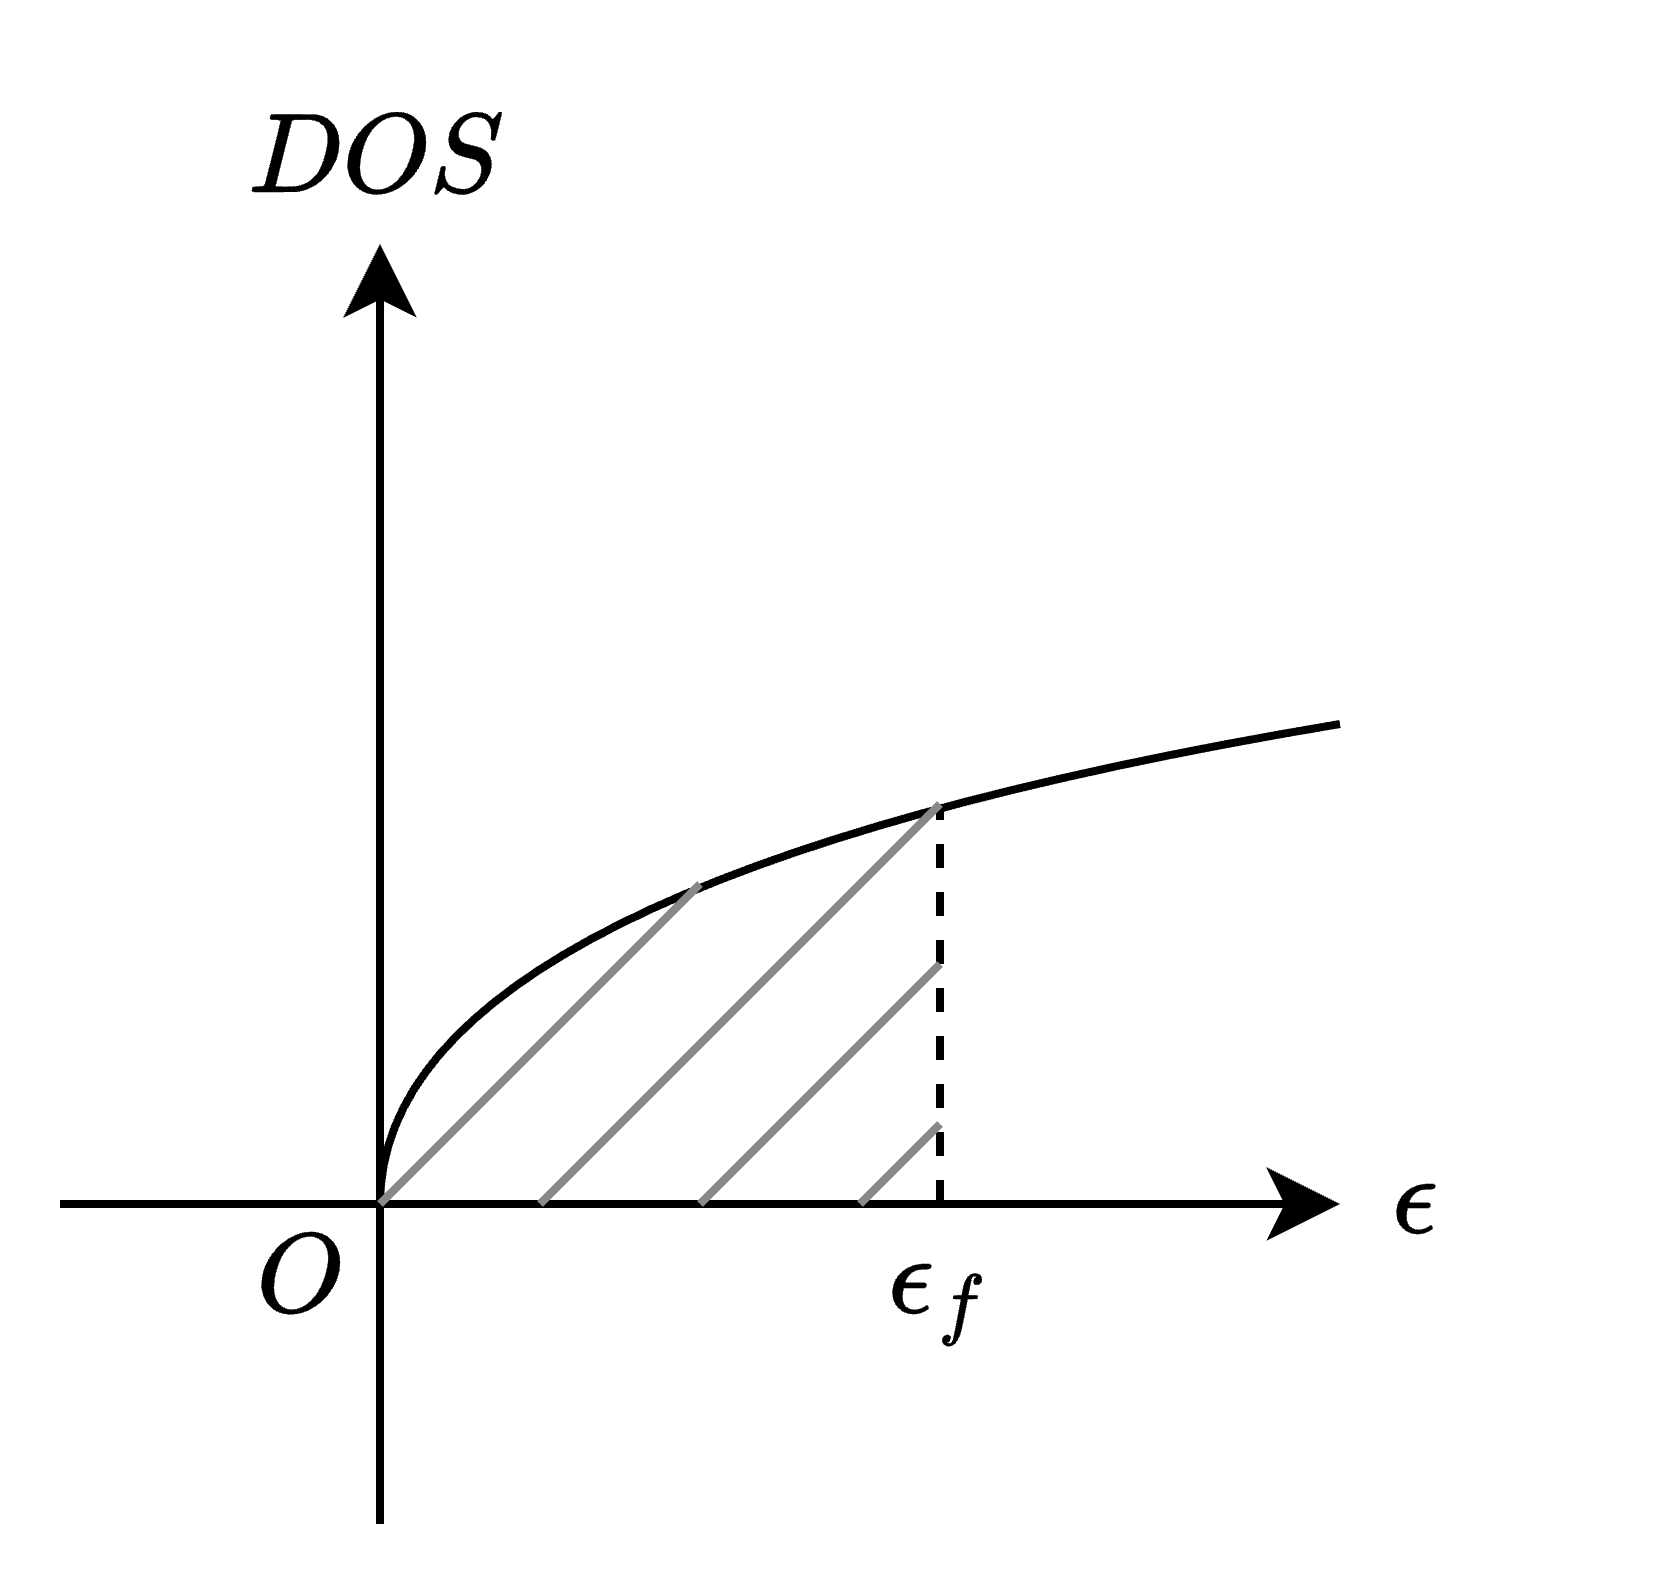
\includegraphics[width=0.4\linewidth]{src/figures/fermi-dirac-distribution/fermi-dirac-distribution.png}
	\caption{フェルミ粒子(電子)のエネルギーとDOSの関係}\label{fig:fermi-dirac-distribution}
\end{figure}

このときDOSは図\ref{fig:fermi-dirac-distribution}のようになる。
金属中では、自由電子のほかに+電荷をもつ陽イオンが規則正しく配列している。
このとき\ref{eq:3d-free-particle}式で表される$k$が小さい場合には陽イオンの影響は無視できるが、
$k$が大きくなり波長が格子間隔$a$に近づいてくると、電子波はブラッグ反射の影響を受けはじめる。
$x$方向の格子間隔$a$の一次元格子を考えると、ブラッグの条件を満足するのは
\begin{equation}
	k = \pm \dfrac{\pi}{a}
\end{equation}
の場合である。

このとき$e^{ikx}$の波が進行するとブラッグ反射で、$-x$方向に$e^{-ikx}$の波が反射されこれらの合成波として
$\sin kx$と$\cos kx$の2種の定常波が可能となる。
このとき図\ref{fig:crystal-wave-function}のようにこう視点の位置で振幅最大のものと最小のものとがあり、
$|\psi|^2$が電子の確率密度を表すことを考えると、陽イオンのところで$|\psi|^2$が最大になる分布はクーロンエネルギーは最小で、
$|\psi|^2$が最小になる波はクーロンエネルギーが最大となる。
\begin{figure}
	\centering
	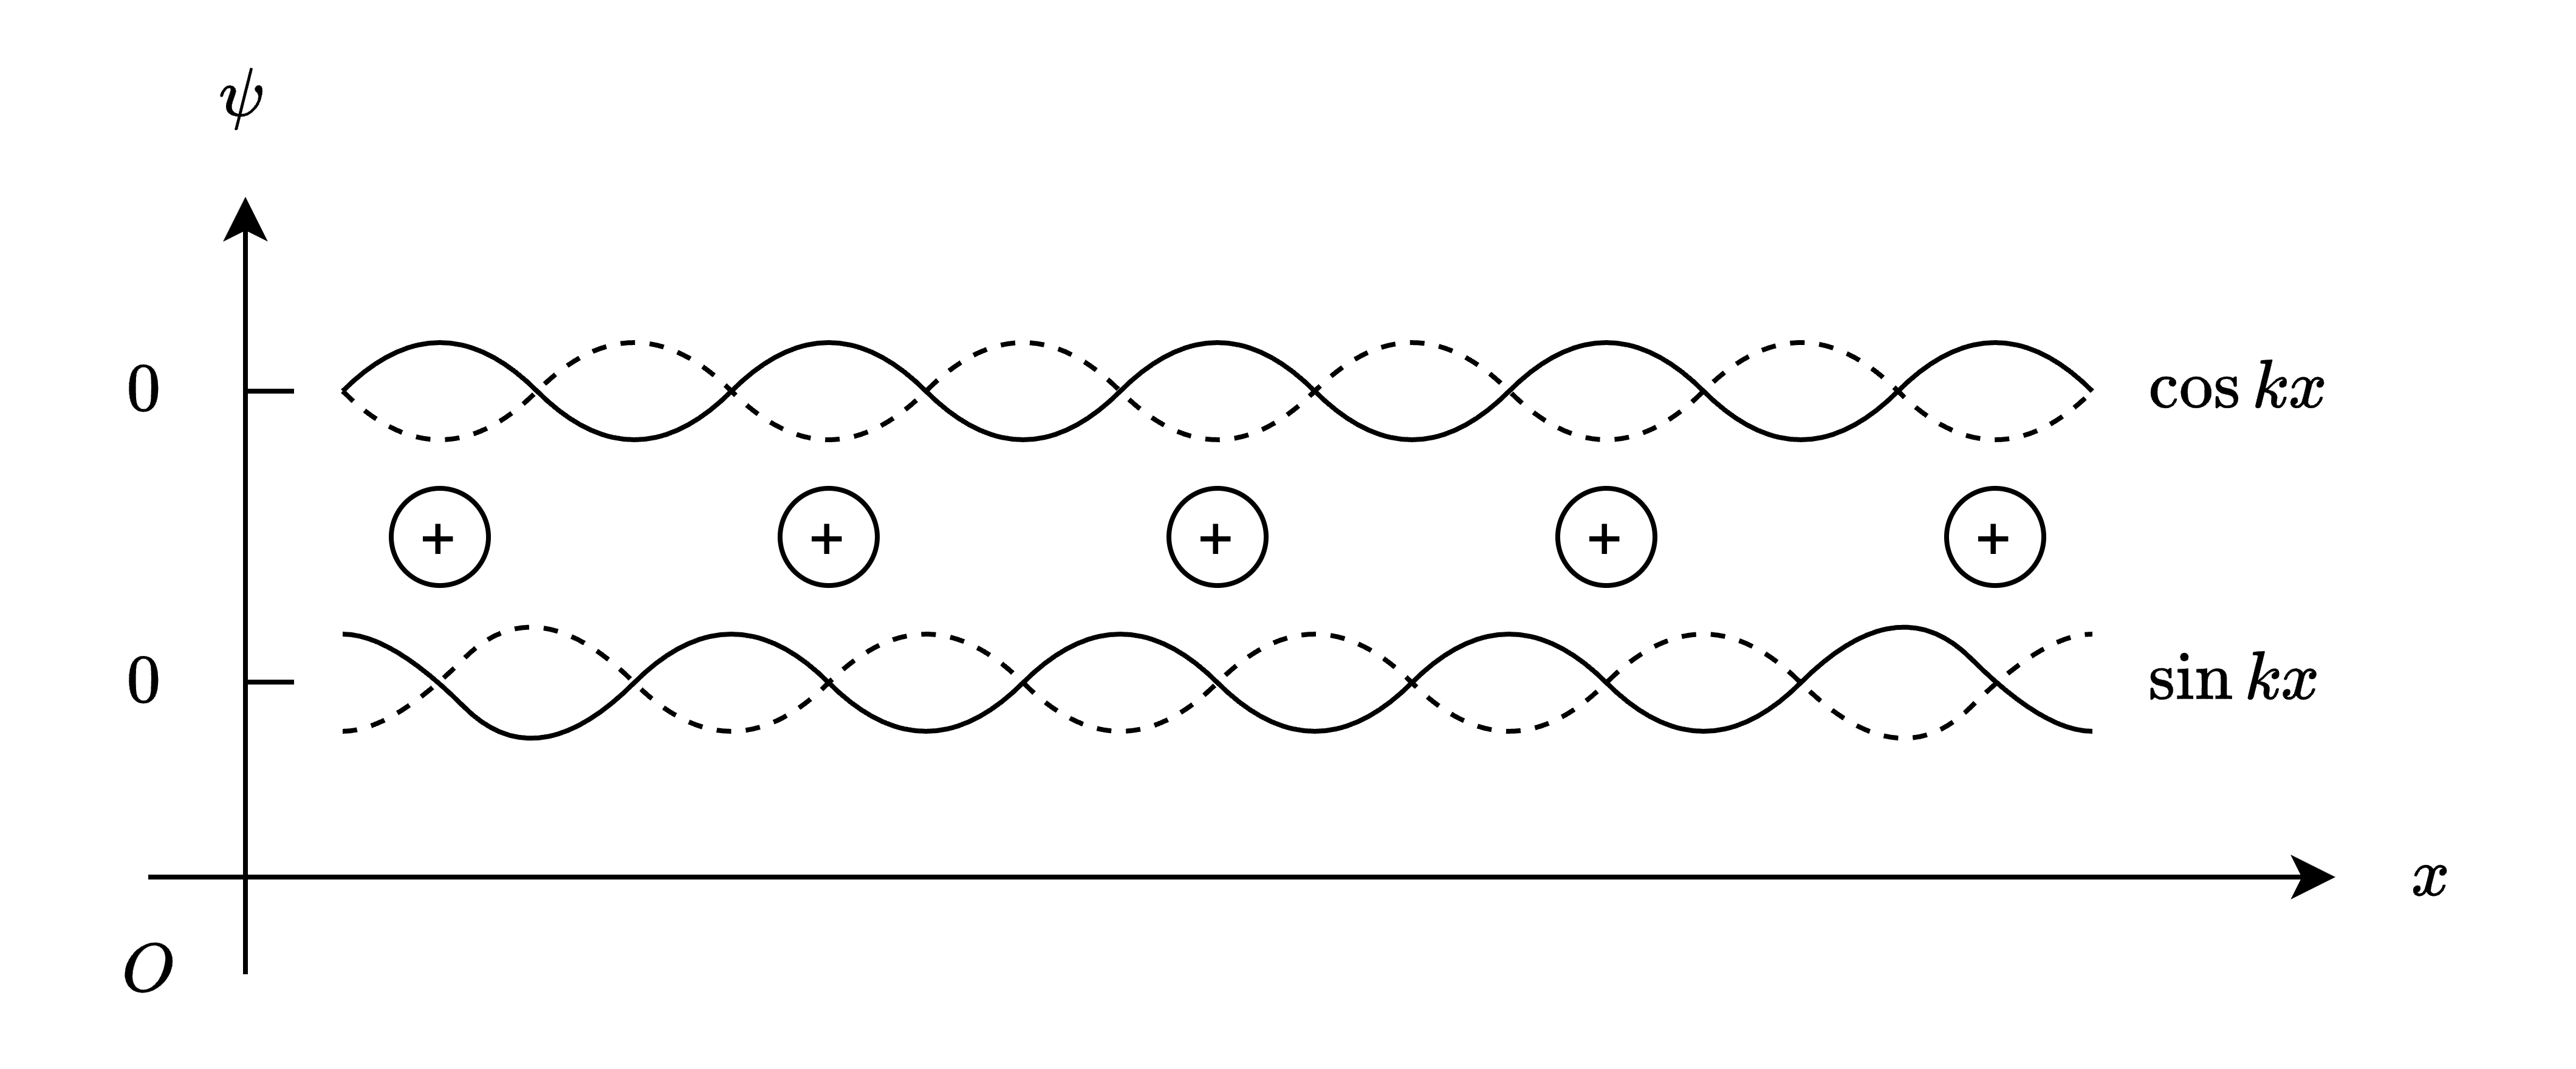
\includegraphics[width=0.6\linewidth]{src/figures/crystal-wave-function/crystal-wave-function.png}
	\caption{結晶中の波動関数の2つの定常波}\label{fig:crystal-wave-function}
\end{figure}

この差を$\Delta \epsilon$とすれば波数に対するエネルギーの曲線、E-k曲線は図\ref{fig:crystal-e-k}のようになり、
$k=\pm \pi/a$のときに$\Delta E$のギャップが生じる。
\begin{figure}
	\centering
	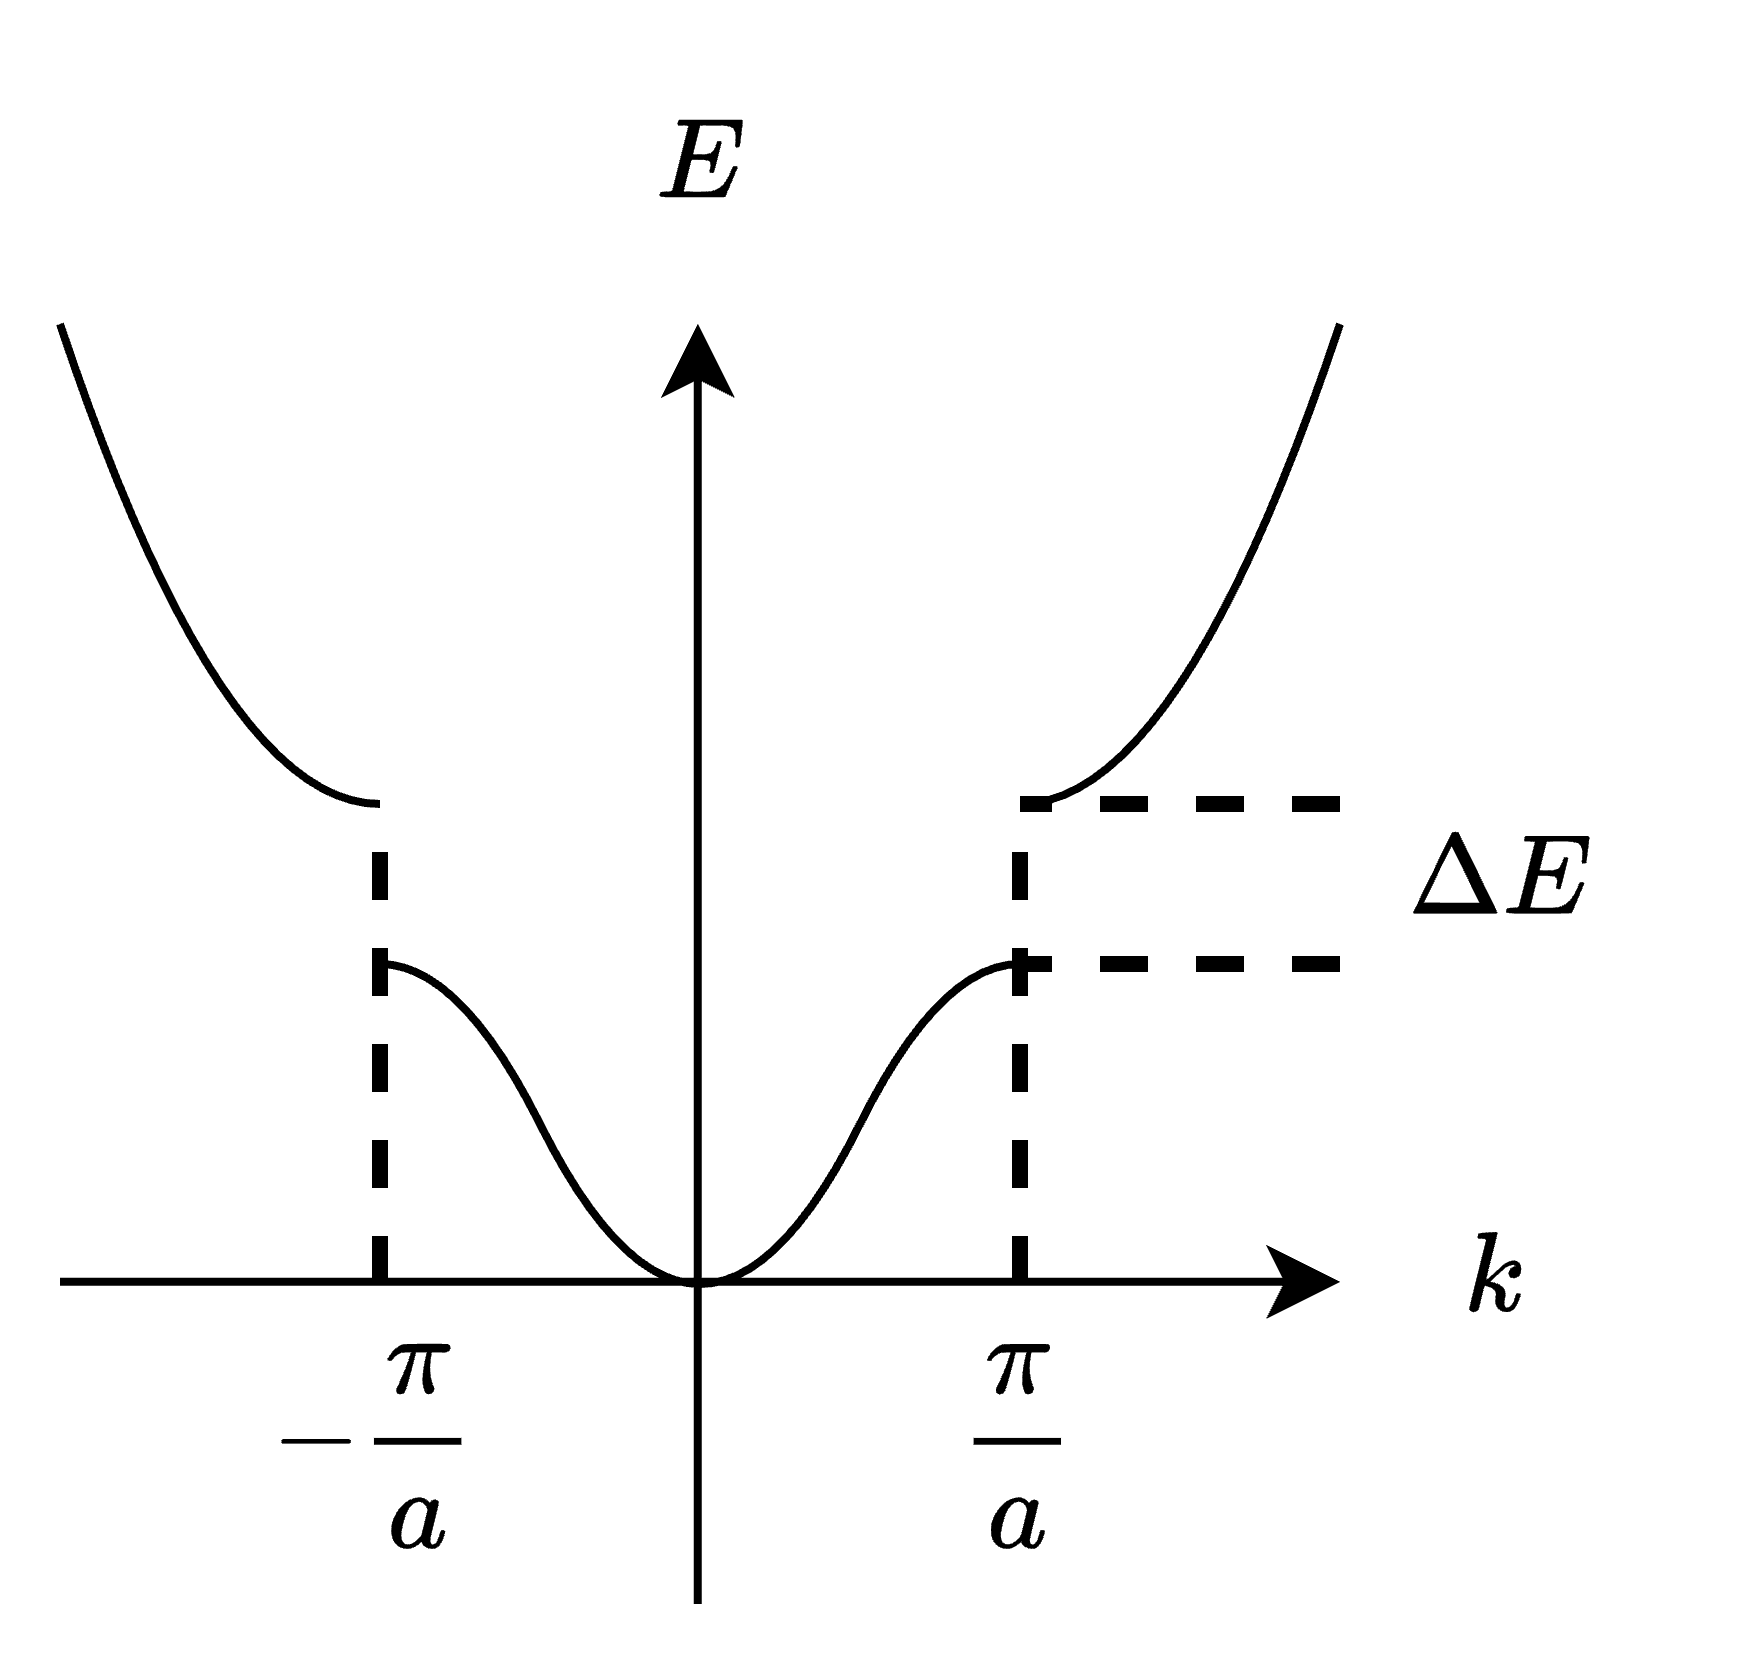
\includegraphics[width=0.4\linewidth]{src/figures/crystal-e-k/crystal-e-k.png}
	\caption{結晶中の電子の$E-k$曲線}\label{fig:crystal-e-k}
\end{figure}

このギャップによって結晶中では状態密度は図\ref{fig:crystal-dos}のように閉じた形となる。
この形で左側にアップスピン、右側にダウンスピンのDOSを描き、外部磁場を加えたときのバンドの分極が起きているときが\ref{fig:tmr-dos}に示したバンド図である。
\begin{figure}
	\centering
	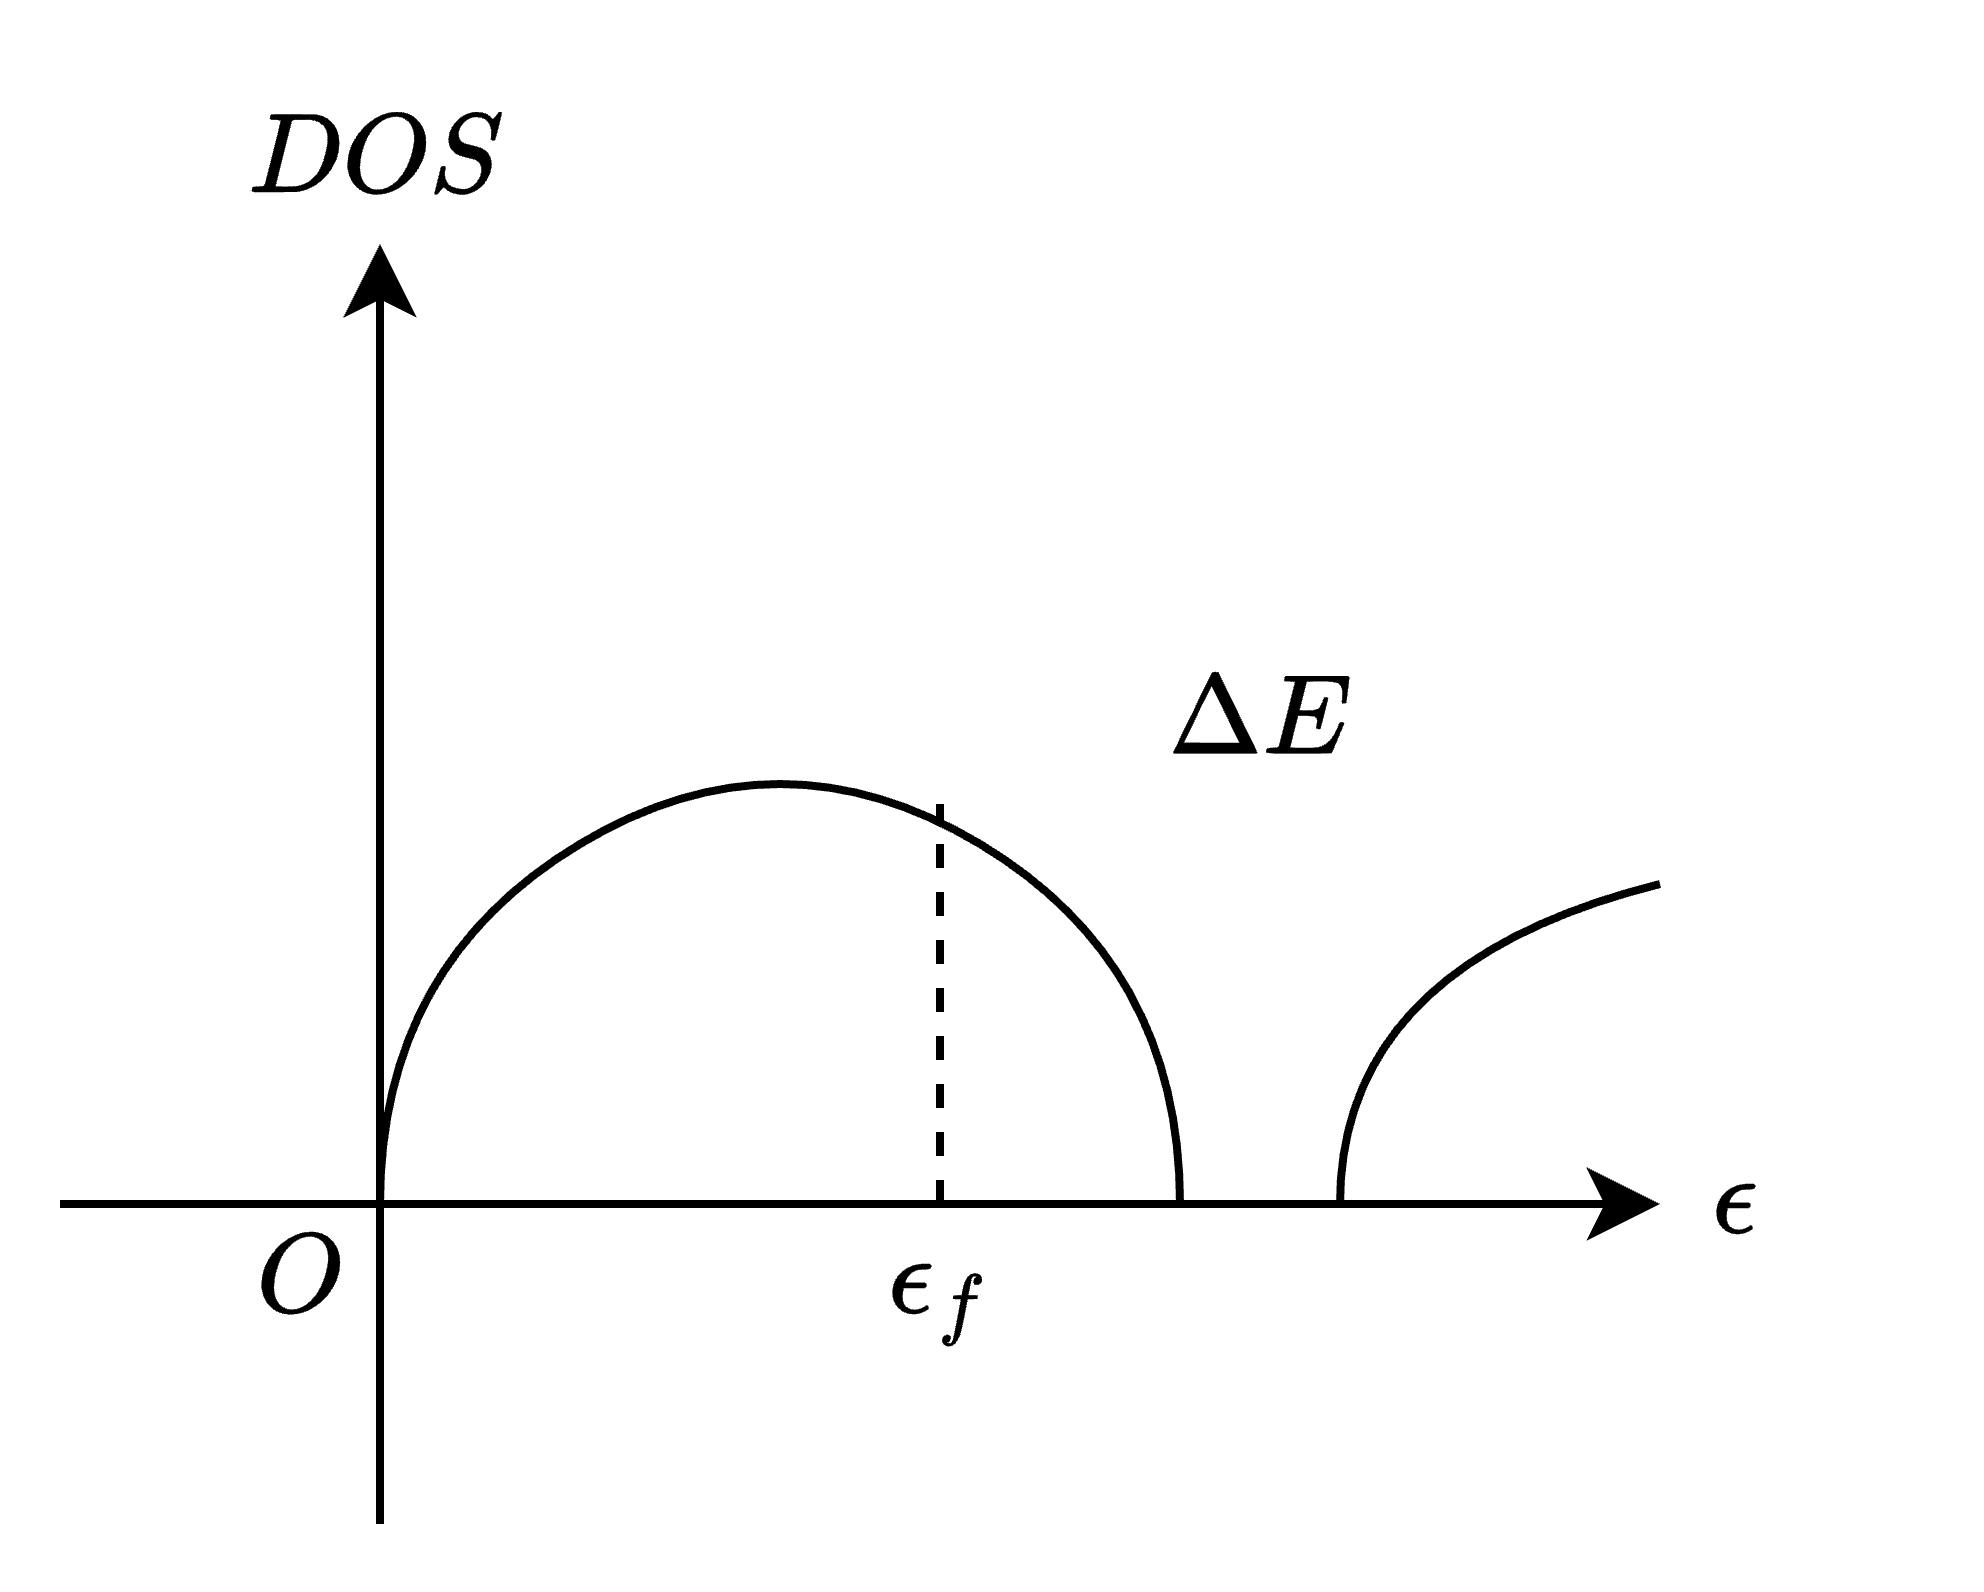
\includegraphics[width=0.6\linewidth]{src/figures/crystal-dos/crystal-dos.png}
	\caption{結晶中のDOS}\label{fig:crystal-dos}
\end{figure}



\subsection{ヒステリシス}\label{subsec:hysteresis}
\ref{subsec:hysteresis-loop}でも述べたように、図\ref{fig:result}では\SI{-7}{A}から\SI{7}{A}までの磁場をかけたときの抵抗の変化と、
\SI{7}{A}から\SI{-7}{A}までの磁場をかけたときの抵抗の変化が異なる。
このことから、MTJ素子はヒステリシス特性を持つとわかる。

ヒステリシスは強磁性体中での結晶磁気異方性と磁区の移動によるものとされている。
磁気異方性とは、強磁性体の自発磁化がその磁性体を形成する特定の結晶軸方向に向きたがる性質\cite{ferromagnetic-2}をいう。
磁区とは、強磁性体内で多くの磁区と呼ばれる部分に分かれていてそれごとに自発磁化の向きが異なる領域をいう。
この磁区はP. Weiss\cite{magnetic-domain}の論文にすでに述べられている。
この磁区ははじめは磁気容易軸にばらばらに向いている(図\ref{subfig:magnetic-domain-before})外部磁場をある方向にかけていくことで全ての軸が同じ方向を向くようになり、磁化が一様になる(図\ref{subfig:magnetic-domain-after})。
この一様磁区になった状態が図\ref{fig:hysteresis-loop}の飽和状態である。
ここから磁場を小さくしていくと核が生成され磁区がいくつか生成されるようになるが、磁場を完全に0にした状態にしても一葉磁区の向いていた方向への磁化は多方向に比べて多く全体として磁化が残る。
これが残留磁化である。
そして外部磁場を逆向きへかけていくことでもとの磁化が0の状態へとなりさらに逆向きの磁場を増やすと、はじめの一様磁区の状態とは逆向きの一様磁化状態へと至る。
これがヒステリシス環線である。
\begin{figure}
    \centering
    \begin{subfigure}{0.48\linewidth}
        \centering
        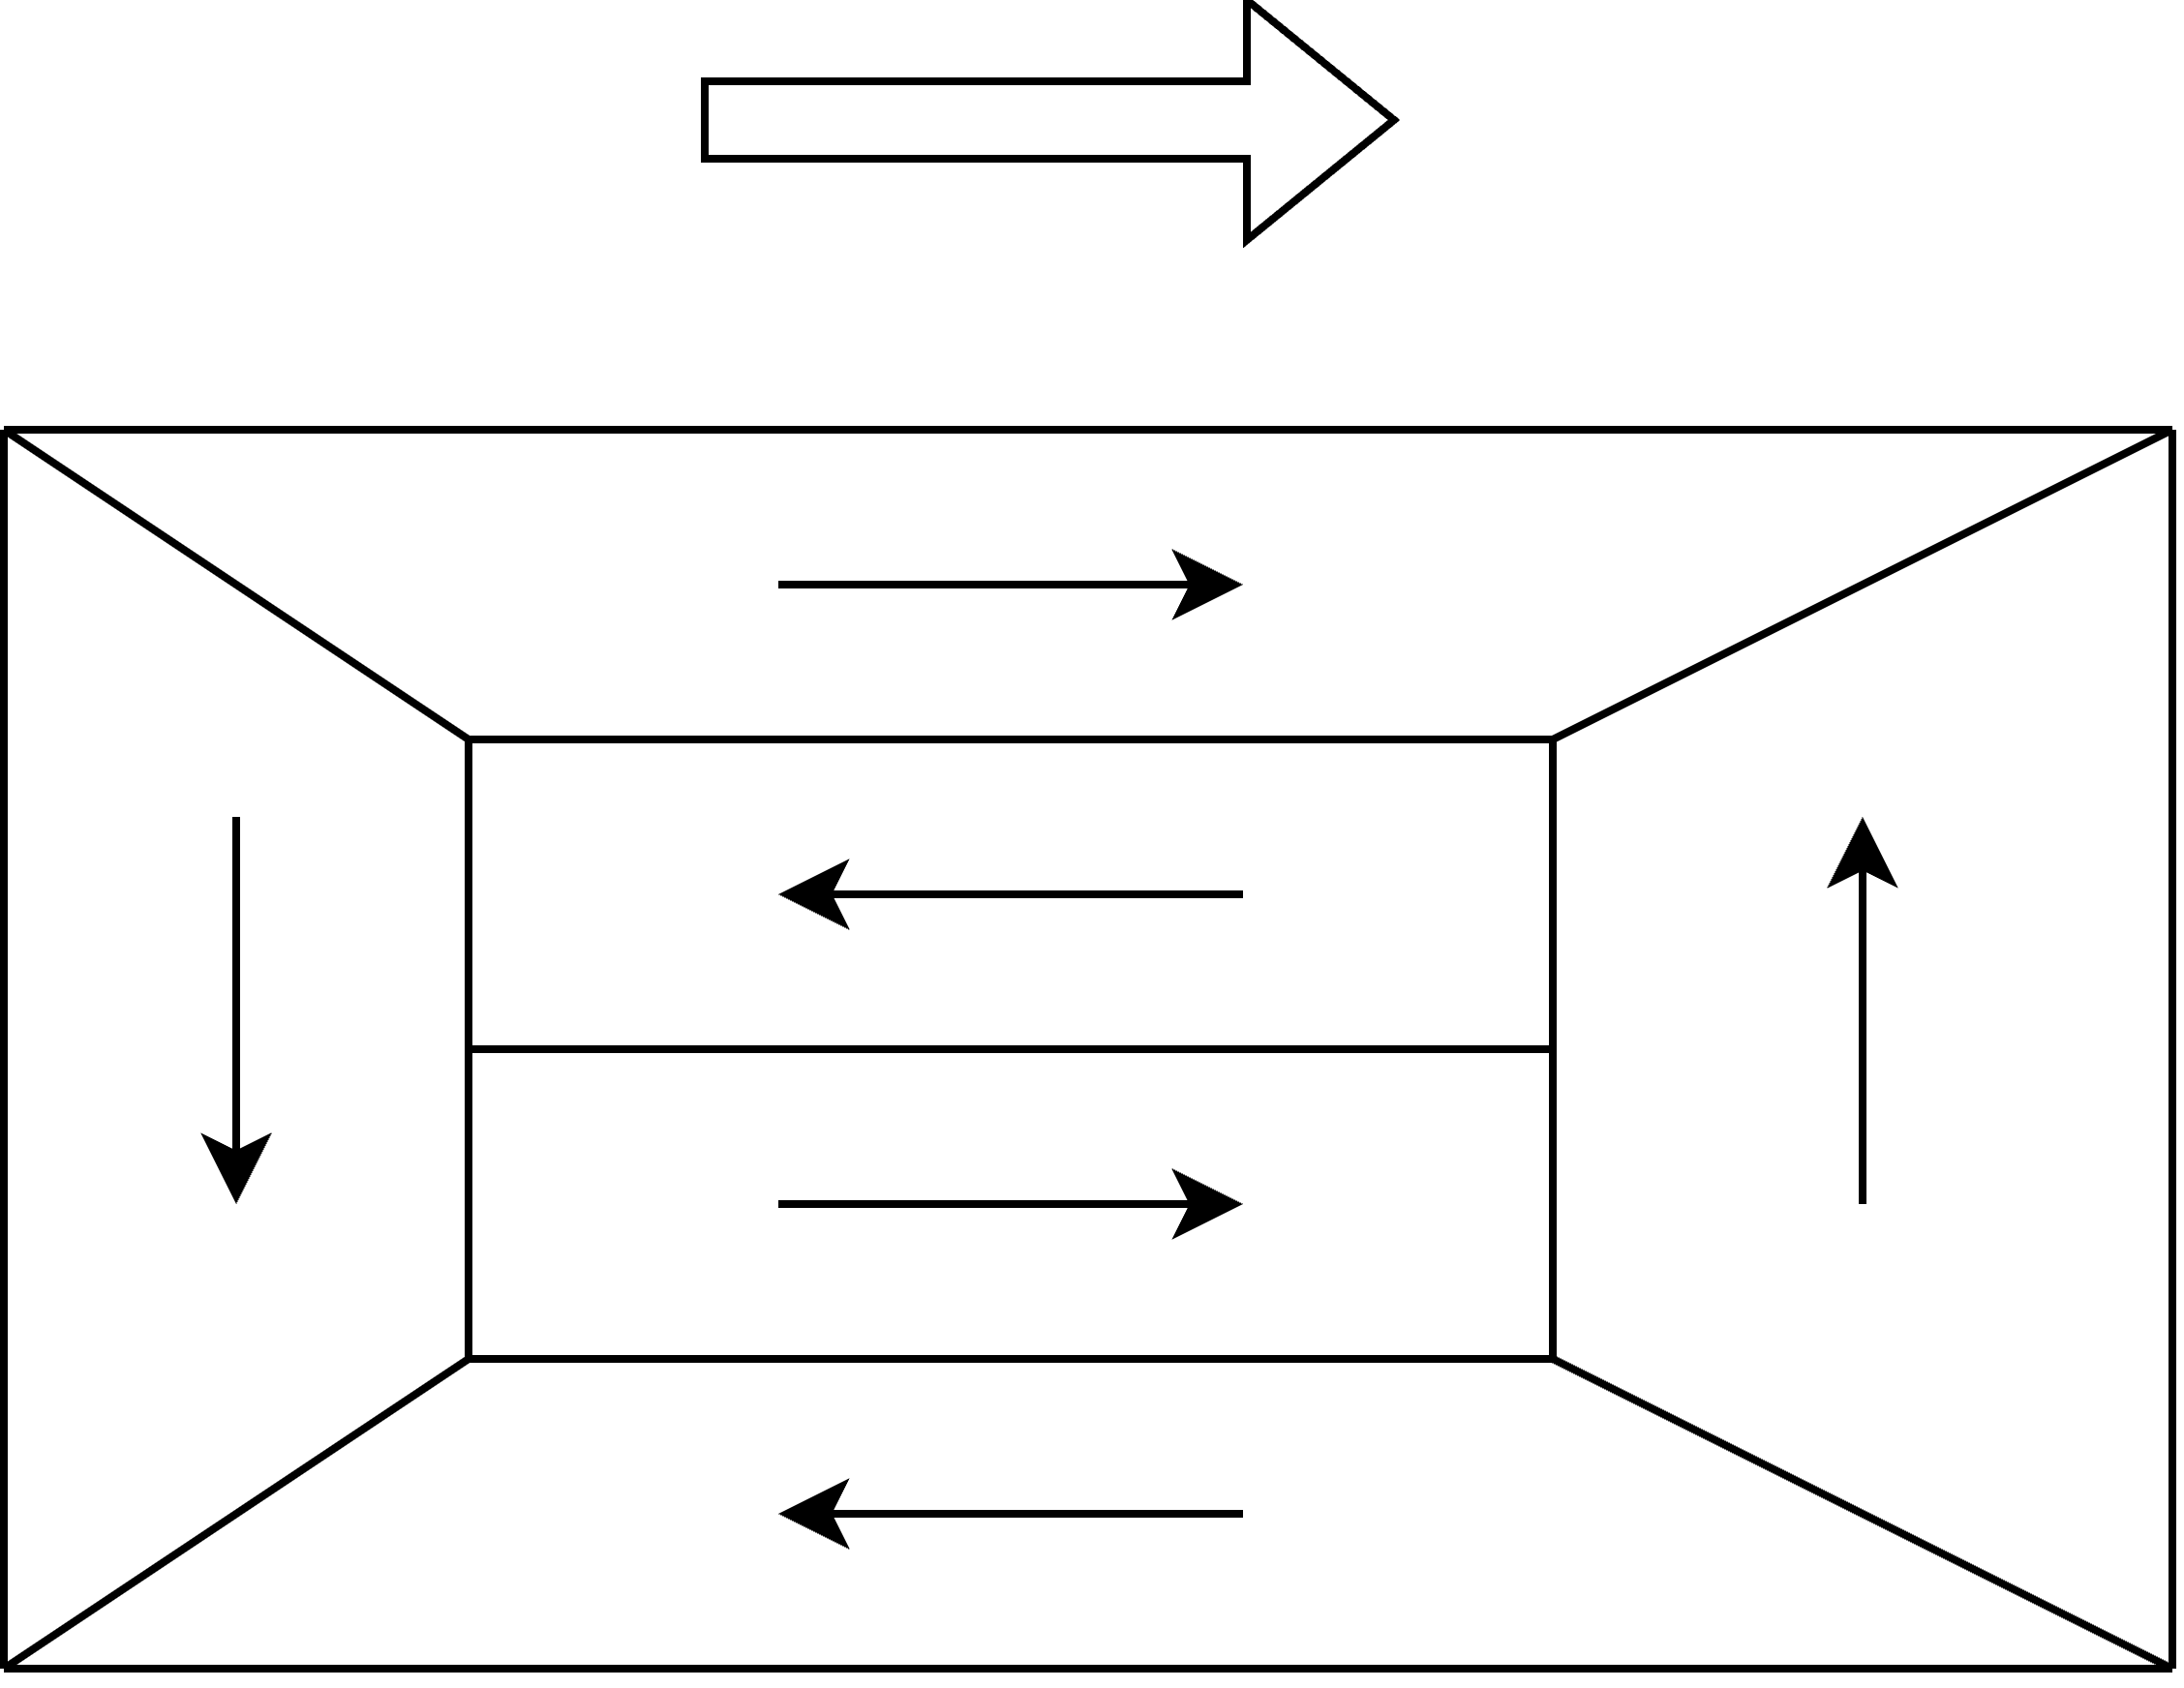
\includegraphics[width=0.8\linewidth]{src/figures/magnetic-domain/magnetic-domain.png}
        \subcaption{磁区(外部磁場をかける前)}\label{subfig:magnetic-domain-before}
    \end{subfigure}
    \begin{subfigure}{0.48\linewidth}
        \centering
        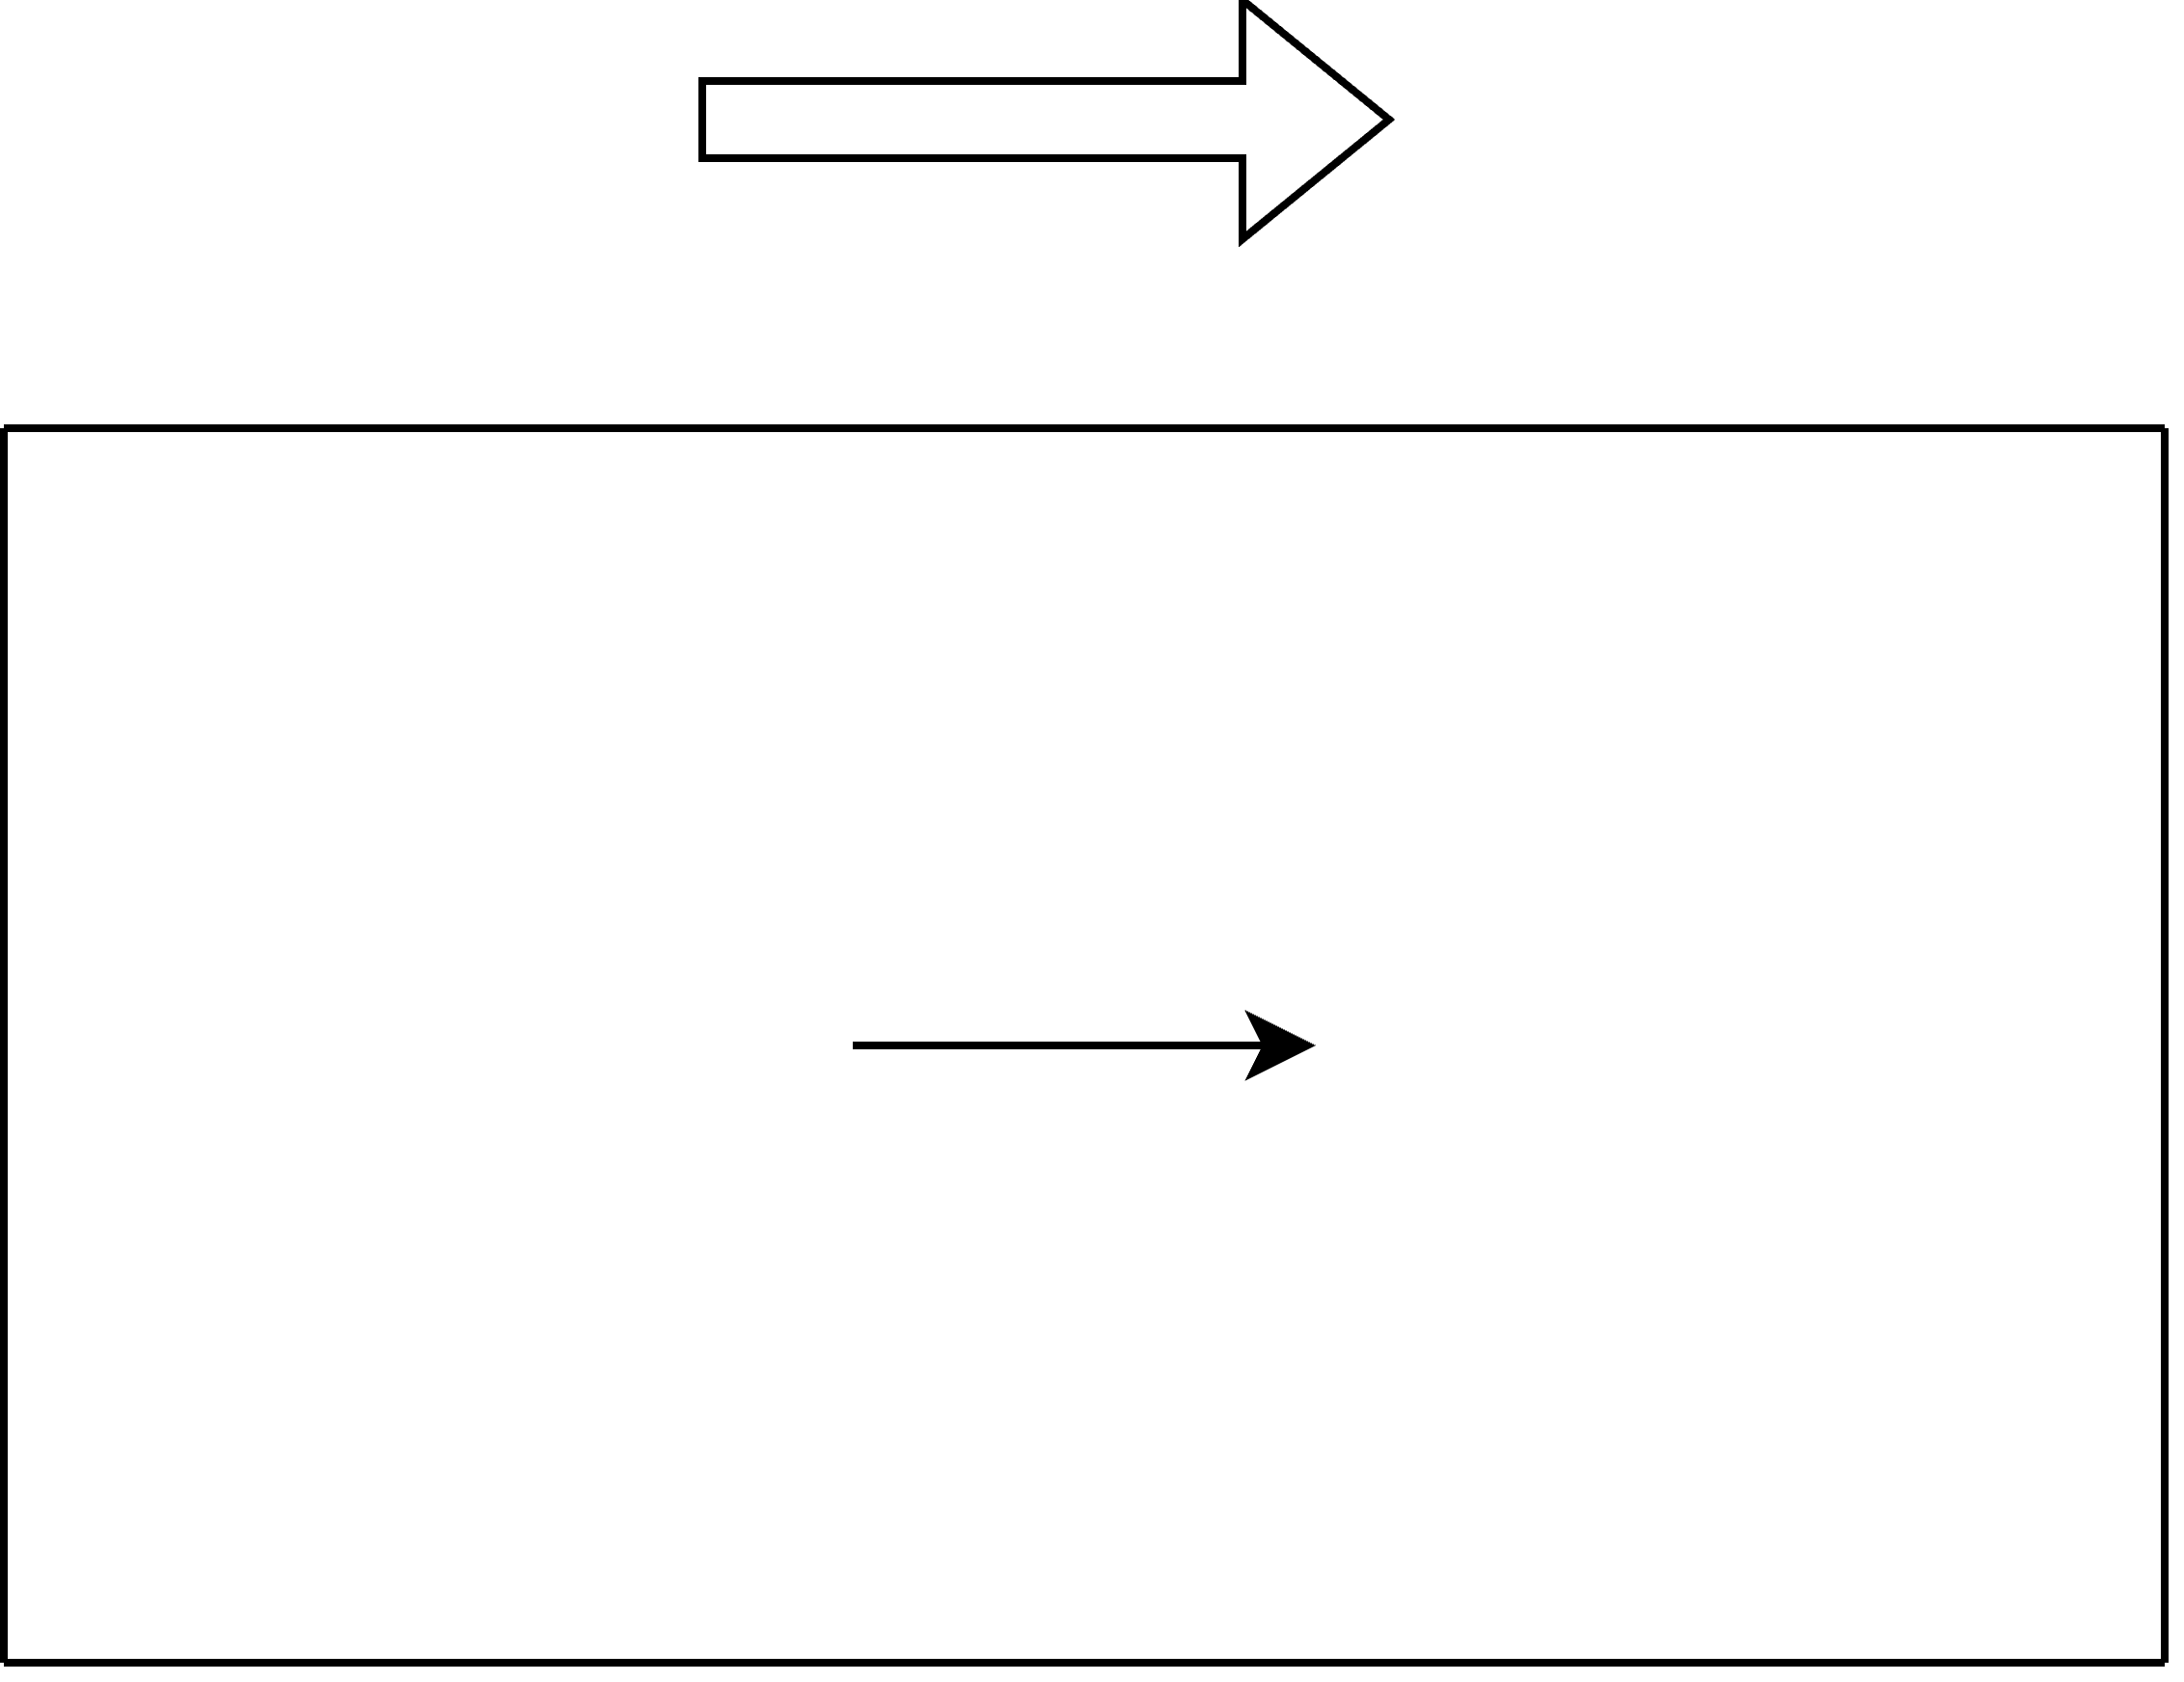
\includegraphics[width=0.8\linewidth]{src/figures/magnetic-domain/magnetic-domain-2.png}
        \subcaption{磁区(一様磁区)}\label{subfig:magnetic-domain-after}
    \end{subfigure}
    \caption{磁区の変化}\label{fig:magnetic-domain}
\end{figure}



\subsection{TMR比}
高感度な磁気ヘッドや磁気センサーの実現には高いTMR比が必要となる。
本実験では、TMR比は\SI{153.5}{\%}でありこれを大きくする方法を考察する。
julliereモデルで考えると、TMR比を大きくするには式\ref{eq:tmr-g-p}と\ref{eq:tmr-g-ap}の差を大きくする必要がある。
磁場に対するバンドの分極の差を大きくする、または磁化の変化を大きくすることが大事と考える。
バンドの分極の差が大きくなればよりMajority SpinとMinority SpinのDOSの差は大きくなりTMR比は大きくなる。
また、\ref{subsec:hysteresis}を踏まえると、磁場に対する磁化は最大値が定まっているが小さい磁場に対して磁化の変化を大きくすることができればより実用的なTMR効果が得られる。
このためには、さまざまな原子で構成される強磁性体の結晶構造を工夫することで磁化の変化を大きくすることができると考えられる。

具体的な手法として、\SI{300}{K}で\SI{604}{\%}のTMR比を達成した\ce{CoFeB}/\ce{MgO}/\ce{CoFeB}というMTJ素子\cite{cofeb-mgo-tmr}では、
この\SI{500}{\celsius}以上でMTJをアニールすることで結晶構造が整えられ、\ce{CoFeB}と\ce{MgO}の界面が整うことで電子のスピントンネル効果が最適化され、
TMR比が大きくなったとある。


\end{document}
